\documentclass[11pt]{article}
\pdfoutput=1
\pdfsuppresswarningpagegroup=1

\usepackage{../../jcapmod}
\input{../../preamble}
\graphicspath{{figures/}}

\begin{document}
\thispagestyle{plain}

\newcommand{\mcmcicon}{%
\raisebox{-0.12ex}{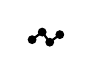
\begin{tikzpicture}[scale=1.6]
    % Random walk path with connected samples
    \fill (0, 0) circle (1.0pt);
    \draw[line width=0.8pt] (0, 0) -- (0.08, 0.06);
    \fill (0.08, 0.06) circle (1.0pt);
    \draw[line width=0.8pt] (0.08, 0.06) -- (0.14, -0.02);
    \fill (0.14, -0.02) circle (1.0pt);
    \draw[line width=0.8pt] (0.14, -0.02) -- (0.22, 0.04);
    \fill (0.22, 0.04) circle (1.0pt);
\end{tikzpicture}}%
}

\chapterheading{\mcmcicon\hspace{0.4em}$\cdot$ MCMC and Variational Inference}

\vspace{1em}
\begin{quote}
\textit{``The generation of random numbers is too important to be left to chance.''}

\raggedleft-- Robert R. Coveyou
\end{quote}
\vspace{0.5em}

\section{You have the posterior. Now what?}

The previous chapter introduced Bayes' theorem:
\beq
\boxed{p(\theta \mid x) = \frac{p(x \mid \theta) \, p(\theta)}{p(x)}}
\eeq
The posterior $p(\theta \mid x)$ is the answer to inference. But the posterior is a \emph{distribution}, not a number. For two parameters, it's a surface. For fifteen parameters, it's a 15-dimensional landscape.

\paragraph{Summaries are integrals.} We rarely need the full distribution. We want summaries: the posterior mean $\E[\theta \mid x]$, credible intervals. Each of these is an integral (Figure~\ref{fig:banana_posterior}):

\begin{figure}[h]
\centering
\begin{minipage}{0.48\textwidth}
\begin{align}
\textcolor{dullred}{\E[\theta \mid x]} &= \int \theta \, p(\theta \mid x) \, d\theta \\[0.5em]
\textcolor{darkgreen}{\Pr(\theta \in [a, b] \mid x)} &= \int_a^b p(\theta \mid x) \, d\theta
\end{align}
\end{minipage}%
\hfill%
\begin{minipage}{0.48\textwidth}
\centering
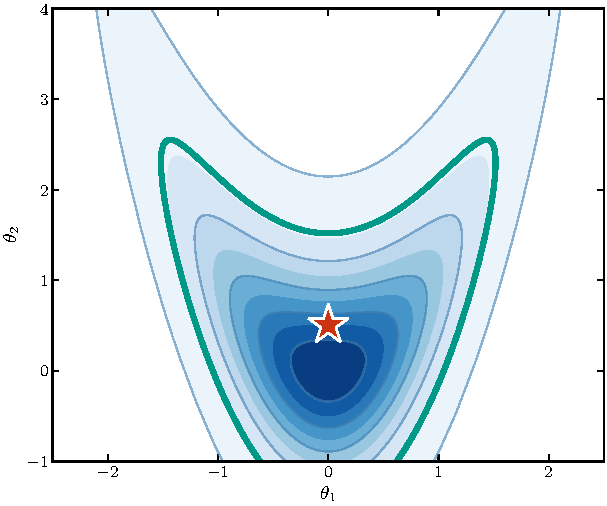
\includegraphics[width=0.95\textwidth]{banana_posterior.pdf}
\end{minipage}
\caption{A two-dimensional posterior distribution. The blue shading shows probability density; darker regions are more probable. The \textcolor{dullred}{red star} marks the posterior mean $\textcolor{dullred}{\E[\theta \mid x]}$. The \textcolor{darkgreen}{green contour} encloses a 95\% credible region $\textcolor{darkgreen}{\Pr(\theta \in R \mid x) = 0.95}$.}
\label{fig:banana_posterior}
\end{figure}

\paragraph{The problem is that we can't do these integrals.} For simple models (like the Gaussian example in Chapter 1), these integrals have closed-form solutions. But for almost any interesting model, they don't. We can \emph{evaluate} the posterior at any point, but we cannot \emph{integrate} it analytically.

% This is the computational bottleneck of Bayesian inference: we have a formula for the posterior, but we're stuck behind integrals we cannot solve.

\paragraph{Two strategies (Figure~\ref{fig:mcmc_vs_vi_intro}).}
\begin{enumerate}
    \item \textbf{MCMC (Markov chain Monte Carlo):} Generate samples from the posterior and replace integrals with averages: $\E[\theta \mid x] \approx \frac{1}{N}\sum_i \theta_i$. Exact in the limit of infinite samples, but can be slow.
    \item \textbf{Variational inference:} Approximate the posterior with a simpler distribution $q(\theta) \approx p(\theta \mid x)$ that we \emph{can} integrate. Fast, but only approximate.
\end{enumerate}

\begin{figure}[h]
\centering
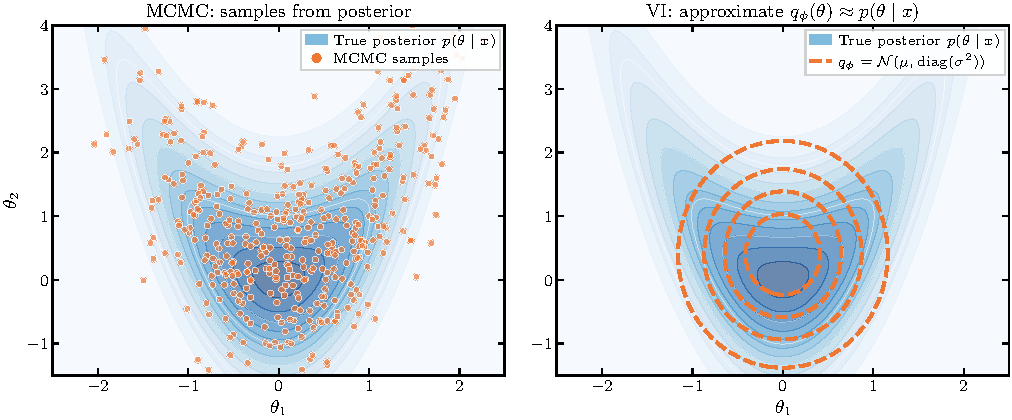
\includegraphics[width=0.95\textwidth]{mcmc_vs_vi_intro.pdf}
\caption{Two approaches to intractable posteriors. The blue shading shows a curved ``banana'' posterior $p(\theta \mid x)$. (Left) MCMC generates samples distributed according to the true posterior, capturing its full structure including correlations. (Right) Variational inference approximates the posterior with a simpler distribution---here a mean-field Gaussian $q_\phi(\theta) = \mathcal{N}(\mu, \mathrm{diag}(\sigma^2))$. The approximation finds the right location but cannot represent the curvature.}
\label{fig:mcmc_vs_vi_intro}
\end{figure}

%% ============================================================
%% PART I: SAMPLING METHODS
%% ============================================================

\section{Monte Carlo integration}

If we had samples from the posterior, we could replace integrals with averages. Suppose we obtain $\theta_1, \theta_2, \ldots, \theta_N \sim p(\theta \mid x)$. Then:
\beq
\E[f(\theta) \mid x] = \int f(\theta) \, p(\theta \mid x) \, d\theta \;\approx\; \frac{1}{N} \sum_{i=1}^N f(\theta_i)
\eeq
The posterior mean is $\bar{\theta} = \frac{1}{N}\sum_i \theta_i$. The variance is the sample variance. A 95\% credible interval comes from sorting the samples and taking the 2.5th and 97.5th percentiles. \textbf{Sampling is just integration/averaging.}

\paragraph{Convergence.} By the law of large numbers, the sample average converges to the true expectation $\E[f(\theta)]$ as $N \to \infty$. The standard error scales as $\sigma / \sqrt{N}$, where $\sigma^2 = \Var[f(\theta)]$. Halving the error requires four times as many samples.

\paragraph{Dimension-free convergence.} The error $\sigma/\sqrt{N}$ depends on $N$ and $\sigma$, but \emph{not on the dimension of $\theta$}. Compare this to grid integration: with 10 points per dimension, a 15D integral needs $10^{15}$ evaluations. Grid methods scale exponentially with dimension. Monte Carlo does not.
%
The catch is that the dimension affects how hard it is to \emph{get} the samples. But once we have them, the averaging is dimension-free.

The main question is the following---how do we sample from a distribution we can only evaluate up to a normalizing constant? We can compute $p(x \mid \theta) p(\theta)$ for any $\theta$, but we don't know $p(x)$, so we can't normalize.

\section{The Metropolis algorithm}

Imagine exploring a landscape where elevation represents probability---higher means more probable (Figure~\ref{fig:mcmc_landscape}). You want to collect samples that represent this landscape (spending more time in high-probability regions), but you can only check elevation where you're standing.

\begin{sciencebox}[Historical note: Arianna Rosenbluth]
The algorithm first appeared in a 1953 paper by Metropolis, the Rosenbluths, and the Tellers. Marshall Rosenbluth later acknowledged that ``Arianna did all the coding''---programming in raw machine language on the MANIAC I computer at Los Alamos. She had earned her PhD in physics from Harvard at 21 (only the fifth woman to do so), after Felix Bloch told her ``flat out, without malice, but just as a fact'' that he wouldn't take female PhD students. She was also a champion fencer who won both women's and men's titles. After Los Alamos, she left physics to raise her children, and when a physicist called in 2003 to ask about the algorithm's development, she was surprised anyone remembered it: ``Oh, that thing.'' More than 50,000 papers have since cited the work. She died in 2020, of COVID-19, at 93.
\end{sciencebox}

\begin{figure}[h]
\centering
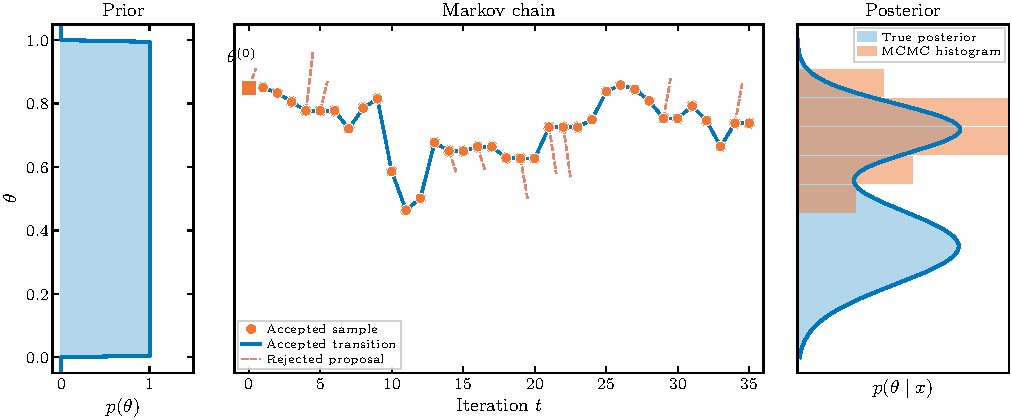
\includegraphics[width=0.95\textwidth]{metropolis_hastings_illustration.pdf}
\caption{The Metropolis algorithm in action. Starting from a uniform prior $p(\theta)$ (left), the algorithm builds a Markov chain (center) by proposing moves and accepting or rejecting them based on the posterior ratio. Accepted proposals (blue lines) move the chain to a new state; rejected proposals (red dashed) leave it in place. After many iterations, the histogram of visited states (orange bars, right) approximates the true posterior $p(\theta \mid x)$ (blue curve).}
\label{fig:mh_illustration}
\end{figure}

\begin{figure}[h]
\centering
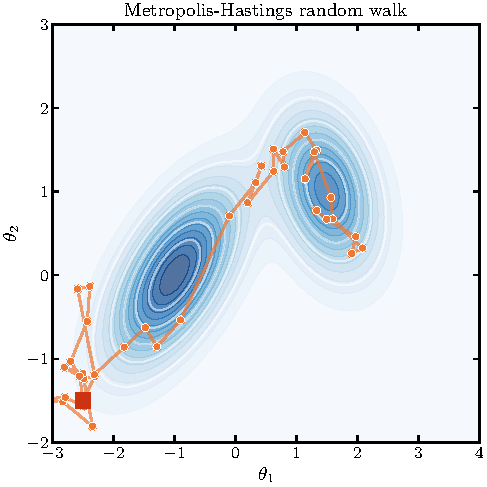
\includegraphics[width=0.7\textwidth]{mcmc_landscape.pdf}
\caption{MCMC as landscape exploration. The surface represents a posterior distribution over two parameters. The algorithm proposes moves (arrows), accepts those that go uphill or pass a random test when going downhill, and traces out a path that spends more time in high-probability regions.}
\label{fig:mcmc_landscape}
\end{figure}

The Metropolis algorithm (Figure~\ref{fig:mh_illustration}) is a random walk with a clever acceptance rule:

\begin{enumerate}
    \item \textbf{Propose:} From current position $\theta$, propose a move to $\theta' \sim \mathcal{N}(\theta, \sigma^2 I)$---a Gaussian centered at the current position.

    \item \textbf{Accept or reject:} Compute the acceptance probability:
    \beq
    \alpha = \min\left(1, \frac{p(\theta' \mid x)}{p(\theta \mid x)}\right)
    \eeq
    If the new spot has higher probability: always accept. If lower: accept with probability $\alpha$.

    \item \textbf{Record:} If accepted, move to $\theta'$; otherwise stay at $\theta$. Record the current position as a sample.
\end{enumerate}

Accepting ``downhill'' moves with probability proportional to the density ratio prevents getting stuck on one peak while still spending more time in high-probability regions.

\subsection{Why does this work?}

Why this particular acceptance rule? The short answer: accepting with probability $\alpha = \min(1, p(\theta')/p(\theta))$ ensures the chain spends time in each region proportional to its probability.

\paragraph{Normalizing constants cancel.} The acceptance ratio only involves $p(\theta' \mid x) / p(\theta \mid x)$. Since both share the same normalizing constant $p(x)$, it cancels:
\beq
\frac{p(\theta' \mid x)}{p(\theta \mid x)} = \frac{p(x \mid \theta') \, p(\theta')}{p(x \mid \theta) \, p(\theta)}
\eeq
We only need the unnormalized posterior---likelihood times prior.

\paragraph{Detailed balance.} The formal justification is \emph{detailed balance}: in equilibrium, the flow of probability between any two states must balance (Figure~\ref{fig:acceptance_intuition}). For states $\theta_A$ and $\theta_B$:
\beq
p(\theta_A) \, T(\theta_A \to \theta_B) = p(\theta_B) \, T(\theta_B \to \theta_A)
\eeq
where $T$ is the transition probability (propose times accept). The Metropolis acceptance ratio makes this hold. Suppose $p(\theta') \geq p(\theta)$. We always accept $\theta \to \theta'$, but only accept $\theta' \to \theta$ with probability $p(\theta)/p(\theta')$. The flows balance:
\beq
p(\theta) \cdot 1 = p(\theta') \cdot \frac{p(\theta)}{p(\theta')} = p(\theta) \quad \checkmark
\eeq

\begin{figure}[h]
\centering
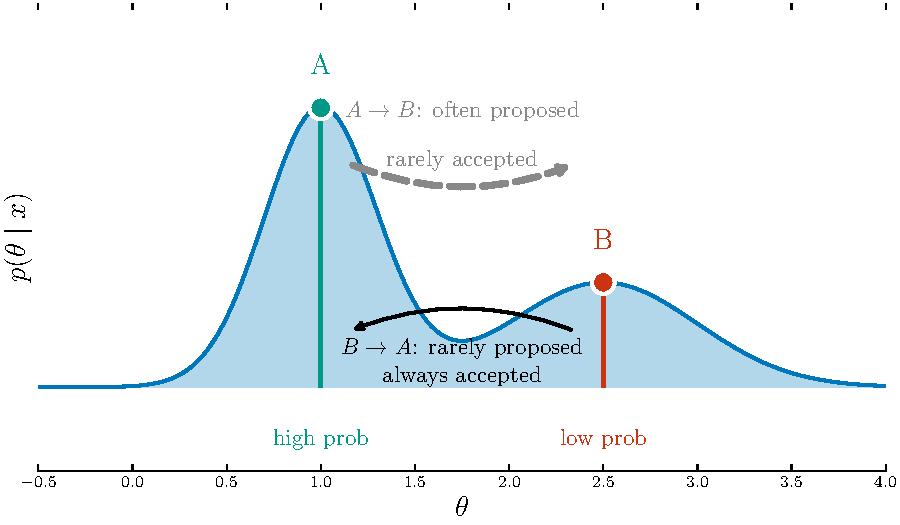
\includegraphics[width=0.95\textwidth]{acceptance_intuition.pdf}
\caption{Detailed balance visualized. In equilibrium, the probability flow from state A to state B exactly balances the flow from B to A. State A has higher probability (darker), so transitions $A \to B$ are always accepted, but $B \to A$ is only accepted with probability $p(A)/p(B)$. The flows balance: $p(A) \cdot T(A \to B) = p(B) \cdot T(B \to A)$. This ensures the chain spends time at each $\theta$ proportional to $p(\theta \mid x)$.}
\label{fig:acceptance_intuition}
\end{figure}

\section{Tuning and convergence}

Efficient MCMC often involves a degree of hyperparameter tuning. The proposal distribution has a free parameter---step size $\sigma$---and getting it right is critical (Figure~\ref{fig:step_size}).

\begin{figure}[h]
\centering
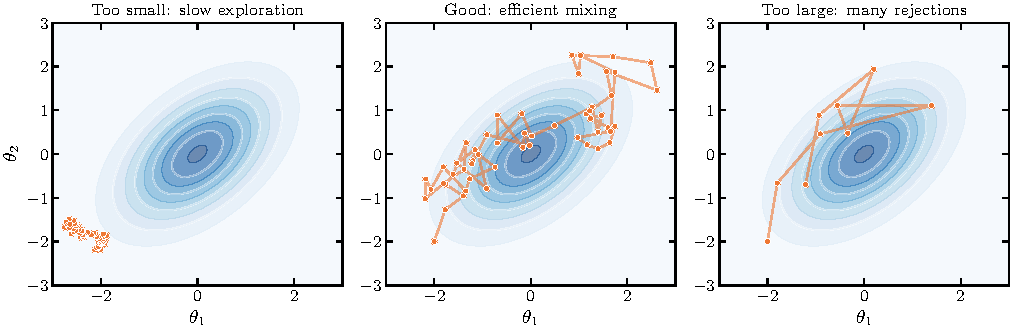
\includegraphics[width=0.85\textwidth]{step_size.pdf}
\caption{The step size tradeoff. (a) Step size too small: nearly all proposals are accepted, but exploration is slow. (b) Step size too large: most proposals land in low-probability regions and are rejected. (c) Step size well-tuned: efficient exploration.}
\label{fig:step_size}
\end{figure}

\begin{itemize}
    \item \textbf{Too small:} Nearly all proposals are accepted, but exploration is slow.
    \item \textbf{Too large:} Most proposals land in low-probability regions and are rejected.
\end{itemize}

A good acceptance rate is roughly 25\% in high dimensions. This is just a heuristic. The intuition: at this rate, the product (acceptance rate) $\times$ (step size) is maximized.

\paragraph{Autocorrelation.} MCMC samples are correlated---each is near the previous. We want to minimize this, since we ideally want a bunch of independent samples which represent our posterior. The \textbf{autocorrelation time} $\tau$ measures how many steps until samples become approximately independent. If $\tau = 100$, then every 100th sample is effectively independent; the effective sample size is $N_{\text{eff}} = N/\tau$ is a proxy for the number of ``independent'' samples.

\section{The failure of random walks in high dimensions}

The random walk Metropolis algorithm scales poorly with dimension. The autocorrelation time grows as $\tau \propto d$---in $d$ dimensions, you need $d$ times more samples to get the same number of ``independent'' samples per dimension.

In high dimensions, probability concentrates in a thin shell called the \emph{typical set} (Figure~\ref{fig:typical_set}). For a $d$-dimensional Gaussian, this shell lies at radius $r \sim \sqrt{d}$ from the mode, with thickness scaling as $1/\sqrt{d}$.

\begin{figure}[h]
\centering
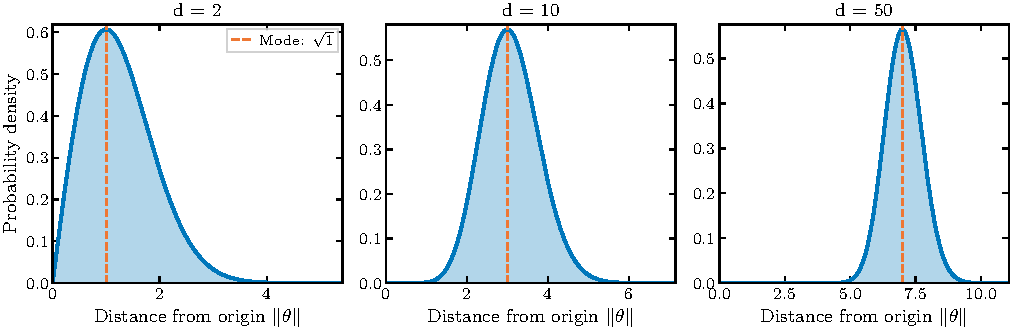
\includegraphics[width=0.95\textwidth]{typical_set.pdf}
\caption{The typical set in high dimensions. For a $d$-dimensional Gaussian, most probability mass lies not at the mode (where density is highest) but in a thin shell at radius $\sqrt{d}$. Volume grows rapidly with radius, overwhelming the density decay.}
\label{fig:typical_set}
\end{figure}

A random walker on this shell faces a geometric problem. To explore the posterior, we need to traverse the shell---move along its surface. But a random walk proposes moves in all directions equally. Most directions point off the shell into low-probability regions.

To stay on the thin shell, we need small step sizes: $\sigma \propto 1/\sqrt{d}$. But then the tangential component---the part that actually explores---also shrinks. The chain makes tiny steps, and autocorrelation time grows as $\tau \propto d$.

\section{Hamiltonian Monte Carlo}

The posterior has structure---the gradient $\nabla \log p(\theta \mid x)$ tells us which way is ``uphill'' (Figure~\ref{fig:gradient_information}). The Metropolis random walk ignores this information. Hamiltonian Monte Carlo (HMC) uses the gradient to make informed, directed moves.

\begin{figure}[h]
\centering
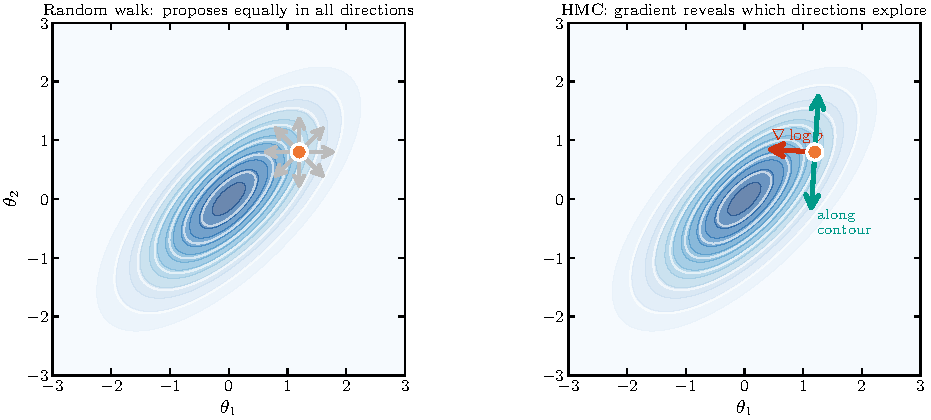
\includegraphics[width=0.95\textwidth]{gradient_information.pdf}
\caption{Why gradients help. (Left) A random walk proposes moves uniformly in all directions. Most directions point off the high-probability region and will be rejected. (Right) The gradient $\nabla \log p(\theta)$ points toward higher probability; directions perpendicular to the gradient are tangent to contours---exactly where we want to move to explore efficiently.}
\label{fig:gradient_information}
\end{figure}

\subsection{The key idea}

The random walk's problem is that it doesn't know which directions stay on the typical set versus which directions point off into low-probability regions. The gradient tells us: $\nabla \log p(\theta)$ points toward higher probability (radially inward), so directions perpendicular to the gradient are tangent to level sets---exactly where we want to move.

But we can't just move perpendicular to the gradient, because that direction changes as we move. We need to \emph{follow} the contours of the distribution as they curve. Physics gives us this: Hamiltonian dynamics.

\subsection{The physics picture}

Imagine a ball rolling on a surface where height is negative log-probability (valleys are high-probability regions). Give the ball a push, and it rolls: speeding up downhill, slowing uphill, curving along the contours. A ball rolling without friction conserves energy---it stays on a single energy level, never drifting into low-probability regions. \textbf{Hamiltonian dynamics naturally traverses level sets of probability!}

Augment parameters $\theta$ with momentum $\rho$. The Hamiltonian (total energy) is:
\beq
H(\theta, \rho) = \underbrace{-\log p(\theta \mid x)}_{\text{potential energy}} + \underbrace{\frac{1}{2}\rho^\top \rho}_{\text{kinetic energy}}
\eeq

Hamilton's equations give the dynamics:
\begin{align}
\frac{d\theta}{dt} &= \rho & \text{(position changes according to momentum)}\\
\frac{d\rho}{dt} &= \nabla \log p(\theta \mid x) & \text{(momentum changes according to gradient)}
\end{align}

\subsection{The algorithm}

\begin{enumerate}
    \item \textbf{Sample momentum:} Draw $\rho \sim \mathcal{N}(0, I)$---give the ball a random push.
    \item \textbf{Simulate dynamics:} Integrate Hamilton's equations for $L$ steps of size $\epsilon$, using the \emph{leapfrog integrator}:
    \begin{align}
    \rho_{t+\epsilon/2} &= \rho_t + \frac{\epsilon}{2} \nabla \log p(\theta_t \mid x) \\
    \theta_{t+\epsilon} &= \theta_t + \epsilon \, \rho_{t+\epsilon/2} \\
    \rho_{t+\epsilon} &= \rho_{t+\epsilon/2} + \frac{\epsilon}{2} \nabla \log p(\theta_{t+\epsilon} \mid x)
    \end{align}
    Leapfrog is \emph{symplectic}: it nearly conserves energy, keeping the acceptance rate high.
    \item \textbf{Metropolis correction:} Accept with probability $\min(1, e^{-H(\theta', \rho') + H(\theta, \rho)})$. True Hamiltonian dynamics conserves energy exactly, so $H(\theta', \rho') = H(\theta, \rho)$ and we'd always accept. But leapfrog uses discrete steps, so energy drifts slightly; the accept-reject step catches proposals where numerical errors pushed us into low-probability regions.
\end{enumerate}

HMC shares the propose-then-accept structure of Metropolis, but differs in two ways:
\begin{itemize}
    \item \textbf{Proposal:} Metropolis draws from a simple distribution (e.g., a Gaussian centered at the current point). HMC simulates Hamiltonian dynamics to generate proposals that follow the posterior's contours.
    \item \textbf{Hyperparameters:} Metropolis has one (step size $\sigma$). HMC has two: step size $\epsilon$ and number of leapfrog steps $L$.
\end{itemize}
The accept-reject criterion has the same form---a ratio of probabilities at the proposed and current points---but HMC's physics-informed proposals achieve high acceptance rates (often ${>}90\%$) even for large moves.

\begin{figure}[h]
\centering
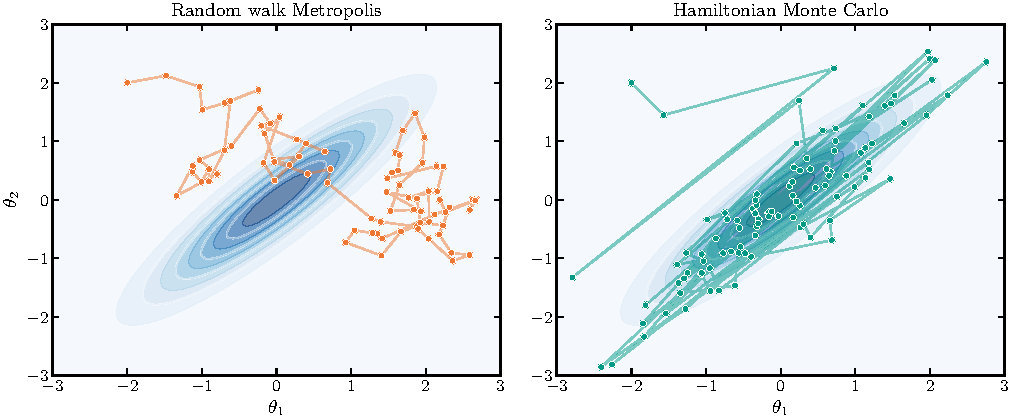
\includegraphics[width=0.9\textwidth]{hmc_vs_rw.pdf}
\caption{Metropolis random walk vs.\ Hamiltonian Monte Carlo. (a) Metropolis: the chain diffuses slowly, taking many small steps. (b) HMC: gradient-informed trajectories make long, directed moves across the posterior.}
\label{fig:hmc_vs_rw}
\end{figure}

Figure~\ref{fig:hmc_vs_rw} compares the two approaches. HMC achieves autocorrelation time $\tau$ nearly independent of dimension---a large improvement over random walk ($\tau \propto d$). The cost is requiring gradients, but automatic differentiation makes this routine.

\section{Diagnostics}

We can never prove MCMC has converged, but failures can often be detected (Figure~\ref{fig:convergence_diagnostics}).

\begin{figure}[h]
\centering
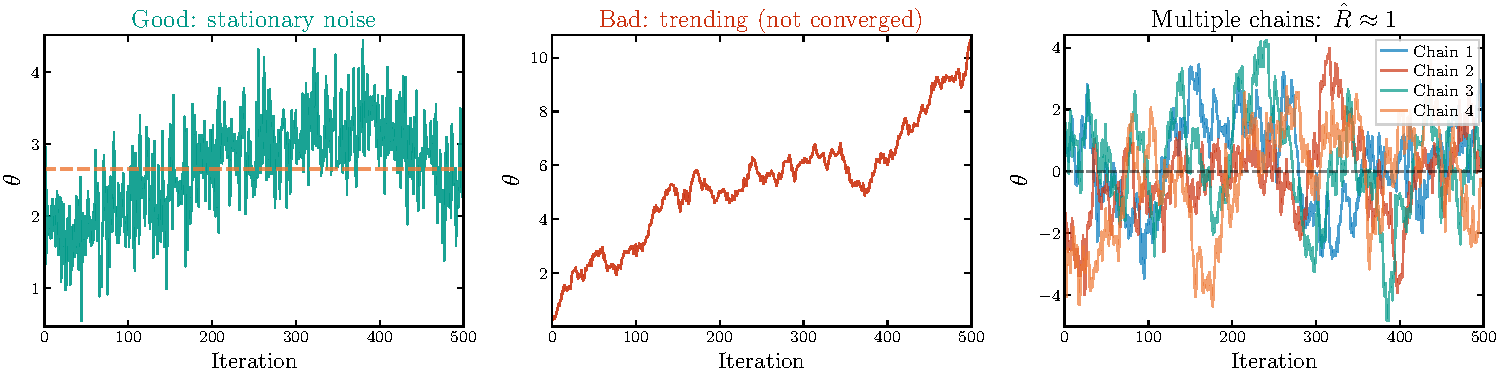
\includegraphics[width=0.95\textwidth]{convergence_diagnostics.pdf}
\caption{MCMC convergence diagnostics via trace plots. (a) Good mixing: the chain fluctuates around a stable mean with no visible trends---this is what we want. (b) Poor mixing: a slow upward drift indicates the chain hasn't reached equilibrium; more samples or better tuning is needed. (c) Multiple chains: running several chains from different starting points that converge to the same distribution is strong evidence of convergence. The $\hat{R}$ statistic formalizes this by comparing within-chain to between-chain variance.}
\label{fig:convergence_diagnostics}
\end{figure}

\paragraph{Trace plots.} Plot each parameter against iteration number. A converged chain looks like stationary noise.

\paragraph{Multiple chains.} Run several chains from different starting points. The $\hat{R}$ statistic compares within-chain variance to between-chain variance; $\hat{R} \approx 1$ indicates agreement.

\paragraph{Effective sample size.} $N_{\text{eff}} = N / \tau$: from $N$ correlated samples, we have information equivalent to $N_{\text{eff}}$ independent ones. Report this, not the raw sample count.

% \section{Using samples}

% Once we have posterior samples, we can answer any question about the posterior.

% \paragraph{Point estimates.} Posterior mean: $\bar{\theta} = \frac{1}{N}\sum_i \theta_i$.

% \paragraph{Credible intervals.} The 16th and 84th percentiles give 68\% credible intervals; 2.5th and 97.5th give 95\%.

% \paragraph{Marginalization is trivial.} To get $p(\theta_1 \mid x)$, just histogram the $\theta_1$ values from your samples. What would be a nightmare integral becomes a one-liner with samples.

% \paragraph{Derived quantities.} For the posterior over some function $g(\theta)$, evaluate $g$ on each sample and histogram the results.

\section{Visualizing high-dimensional posteriors}

In real problems, the posterior lives in many dimensions.

\paragraph{Corner plots.} The standard visualization is the \emph{corner plot}: a grid showing all pairwise 2D marginals (off-diagonal) and 1D marginals (diagonal). Each dot in the 2D panels is an MCMC sample; the contours are smoothed density estimates (typically kernel density estimation) enclosing 68\% and 95\% of the probability mass. The diagonal panels show histograms of each parameter's marginal distribution. With thousands of samples, the histogram bins and density contours converge to the true marginal posteriors.

Figure~\ref{fig:corner_cosmology} shows a corner plot from the Planck satellite, which measured the cosmic microwave background---light from 380,000 years after the Big Bang. Cosmologists ran MCMC to infer parameters like the expansion rate $H_0$ and matter density $\Omega_m$ from these measurements. The tilted contours in the $H_0$--$\Omega_m$ panel reveal a degeneracy: many combinations of expansion rate and matter density fit the data equally well. This correlation would be invisible if we only reported the marginal means and standard deviations.

Corner plots reveal degeneracies (tilted ellipses), multimodality (multiple peaks), and non-Gaussianity (asymmetric marginals) that summary statistics hide.

\begin{figure}[!h]
\centering
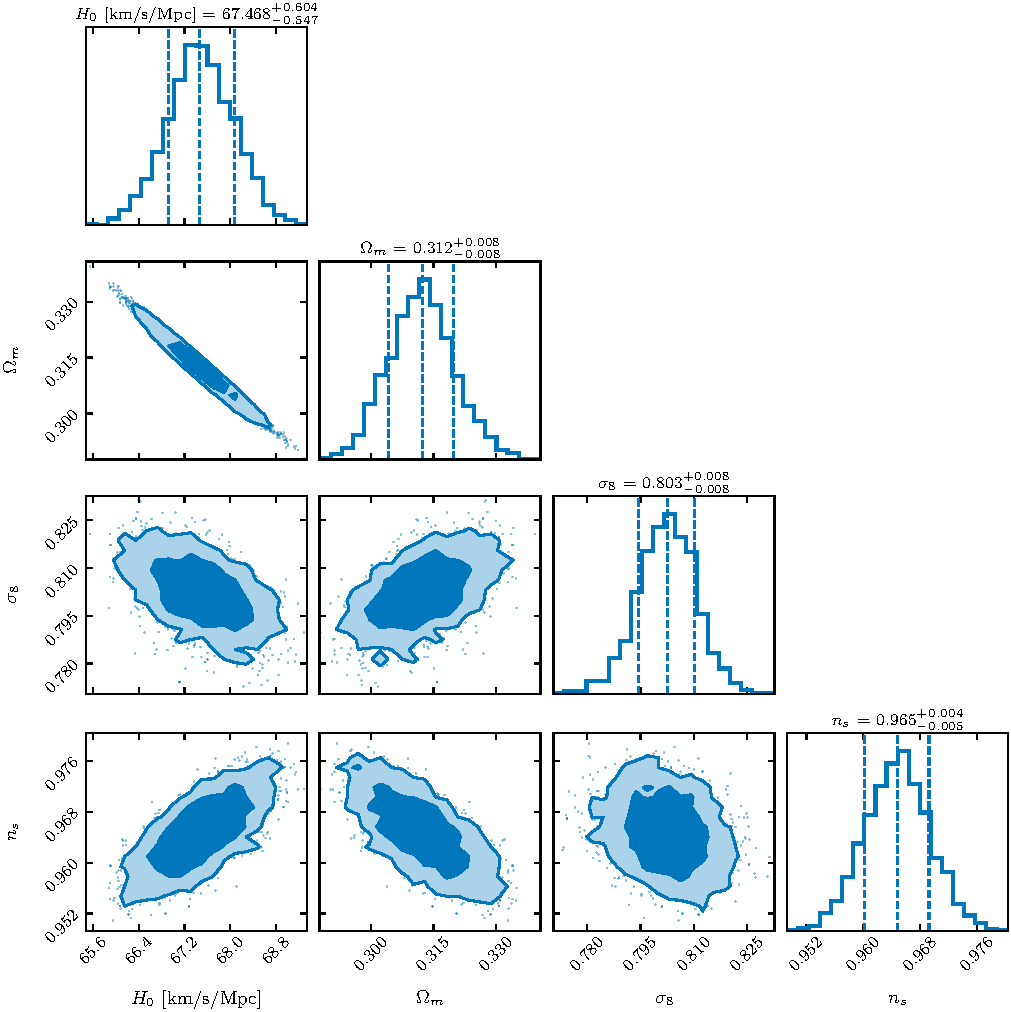
\includegraphics[width=0.85\textwidth]{corner_cosmology.pdf}
\caption{Corner plot from the Planck satellite's measurement of the cosmic microwave background (CMB)---the afterglow of the Big Bang. The Planck collaboration ran MCMC to estimate cosmological parameters from temperature and polarization fluctuations in the CMB; samples shown here are from the PR4 data release. Parameters shown: Hubble constant $H_0$ (expansion rate today), matter density $\Omega_m$, fluctuation amplitude $\sigma_8$, and spectral index $n_s$ (how fluctuations vary with scale). The $H_0$--$\Omega_m$ anticorrelation arises because both affect the angular diameter distance to the CMB. Contours show 68\% and 95\% credible regions. Data from \href{https://arxiv.org/abs/2302.12911}{Lemos \& Lewis (2023)}.}
\label{fig:corner_cosmology}
\end{figure}
%% ============================================================
%% PART II: VARIATIONAL INFERENCE
%% ============================================================

\section{Variational inference}

MCMC gives exact samples but can be slow---especially for models with many parameters or applications requiring real-time inference.

Variational inference (VI) trades exactness for speed by approximating the posterior with a simpler (usually parameterized) distribution, turning inference into optimization of those parameters.

\paragraph{The idea.} Choose a family $\mathcal{Q}$ of tractable distributions (e.g., Gaussians) and find the member $q^*$ that best approximates the true posterior (Figure~\ref{fig:vi_geometry}).

\begin{figure}[h]
\centering
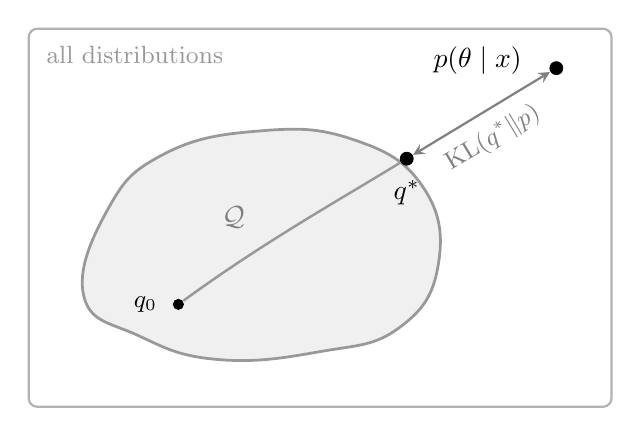
\begin{tikzpicture}[
    dot/.style={circle, fill=black, inner sep=0pt, minimum size=5pt},
    smalldot/.style={circle, fill=black, inner sep=0pt, minimum size=4pt},
]
    % Outer rectangle: space of all distributions
    \draw[black!30, line width=0.8pt, rounded corners=3pt] (-3.2,-2.0) rectangle (4.2,2.8);
    \node[anchor=north west, black!40] at (-3.1,2.7) {\small all distributions};

    % Blobby region for variational family Q
    \path[draw=black!40, fill=black!6, line width=1pt]
      plot[smooth cycle, tension=0.75]
      coordinates{
        (-2.5,-0.6) (-2.2,0.5) (-1.5,1.2) (-0.3,1.5) (0.9,1.4)
        (1.8,0.8) (2.0,-0.2) (1.5,-1.0) (0.5,-1.3) (-0.8,-1.4) (-1.8,-1.1)
      };

    % Family label
    \node[black!50] at (-0.6,0.4) {$\mathcal{Q}$};

    % True posterior (outside Q, in upper right)
    \node[dot] (ptrue) at (3.5,2.3) {};
    \node[anchor=south] at (2.5,2.1) {$p(\theta \mid x)$};

    % Optimal point (on boundary of Q)
    \node[dot] (qstar) at (1.6,1.15) {};
    \node[anchor=north] at (1.6,1.0) {$q^*$};

    % Initial point (inside Q)
    \node[smalldot] (qinit) at (-1.3,-0.7) {};
    \node[anchor=east] at (-1.45,-0.7) {\small $q_0$};

    % Optimization path (curved, inside Q)
    \draw[black!40, line width=0.9pt]
      (qinit) .. controls (-0.2,0.1) and (0.7,0.6) .. (qstar);

    % KL divergence (double-headed arrow showing distance)
    \draw[black!50, <->, >=stealth, line width=0.8pt] (qstar) -- (ptrue);
    % KL label below the line
    \node[black!50, anchor=north, rotate=31] at (2.55,1.65) {\small $\mathrm{KL}(q^* \| p)$};
\end{tikzpicture}
\caption{The geometry of variational inference. The outer box is the space of all distributions; the shaded region is the variational family $\mathcal{Q}$. The true posterior $p(\theta \mid x)$ lies outside $\mathcal{Q}$. Starting from an initial approximation $q_0$, we optimize to find $q^*$---the member of $\mathcal{Q}$ closest to the true posterior, minimizing the KL divergence (dashed).}
\label{fig:vi_geometry}
\end{figure}

\paragraph{Measuring closeness.} The Kullback--Leibler divergence measures how different two distributions are (Figure~\ref{fig:kl_divergence}):
\beq
\KL(q \| p) = \int q(\theta) \log \frac{q(\theta)}{p(\theta \mid x)} \, \d\theta
\eeq
\begin{figure}[h]
\centering
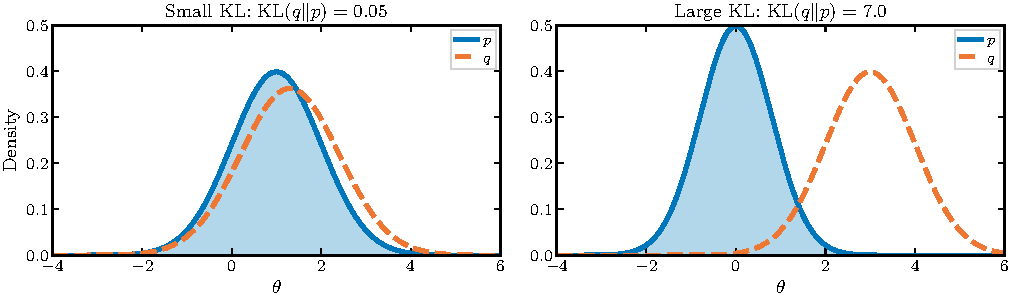
\includegraphics[width=0.9\textwidth]{kl_divergence.pdf}
\caption{KL divergence measures how different two distributions are. (Left) When $q$ and $p$ are similar, KL is small. (Right) When $q$ places mass where $p$ is nearly zero, KL is large---the $\log(q/p)$ term blows up.}
\label{fig:kl_divergence}
\end{figure}

We want $q^* = \argmin_{q \in \mathcal{Q}} \KL(q(\theta) \| p(\theta \mid x))$. But computing the KL requires the normalizing constant $p(x)$---exactly the intractable integral we're trying to avoid.

\section{The evidence lower bound (ELBO)}

\paragraph{What we can and can't compute.} We can evaluate the joint $p(x, \theta) = p(x \mid \theta) p(\theta)$ for any $\theta$. We cannot compute the marginal $p(x) = \int p(x, \theta) \, d\theta$. The ELBO lets us optimize using only the joint.

The key identity is:
\beq
\log p(x) = \text{ELBO}(q) + \KL(q \| p)
\eeq
where $\text{ELBO}(q) = \E_q[\log p(x, \theta)] - \E_q[\log q(\theta)]$.

Since $\KL \geq 0$, the ELBO is a lower bound on the log-evidence:
\beq
\text{ELBO}(q) \leq \log p(x)
\eeq
And since $\log p(x)$ is constant with respect to $q$:
\beq
\boxed{\argmax_q \text{ELBO}(q) \;=\; \argmin_q \KL(q \| p)}
\eeq
So maximizing the ELBO is equivalent to minimizing the KL divergence. The ELBO only involves the joint $p(x, \theta) = p(x \mid \theta) p(\theta)$---no normalizing constant needed. And we also get the log-evidence lower bound ``for free.''

\section{The two forces in the ELBO}

The ELBO can be rewritten as:
\beq
\boxed{\text{ELBO}(q) = \underbrace{\E_{q}[\log p(x \mid \theta)]}_{\text{expected log-likelihood}} - \underbrace{\KL(q(\theta) \| p(\theta))}_{\text{divergence from prior}}}
\eeq

\begin{figure}[h]
\centering
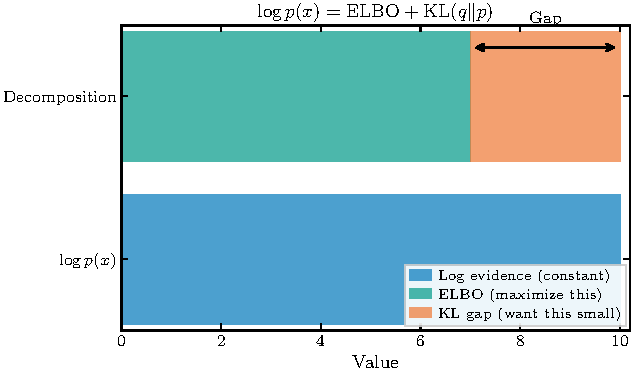
\includegraphics[width=0.85\textwidth]{elbo_decomposition.pdf}
\caption{The two terms in the ELBO. The expected log-likelihood rewards $q$ for placing mass where the data are well-explained. The KL from prior penalizes deviation from prior beliefs.}
\label{fig:elbo_decomposition}
\end{figure}

Two opposing forces (Figure~\ref{fig:elbo_decomposition}): the first term rewards $q$ for concentrating on parameters that explain the data well; the second penalizes $q$ for deviating from the prior. The optimal $q$ balances these pressures.

\section{Optimizing the ELBO}

The variational distribution $q(\theta; \phi)$ is parameterized by $\phi$ (e.g., means and variances for a Gaussian). We maximize the ELBO with respect to $\phi$ using gradient ascent.

\begin{sciencebox}[Computing gradients (optional)]
The challenge is that the ELBO involves an expectation over $q$, which depends on $\phi$---we need to differentiate through an expectation whose distribution depends on the parameters.

\textbf{The reparameterization trick.} Write samples as a deterministic transformation of fixed noise. For a Gaussian $q(\theta; \mu, \sigma) = \mathcal{N}(\mu, \sigma^2)$:
\beq
\theta = \mu + \sigma \cdot \epsilon, \quad \epsilon \sim \mathcal{N}(0, 1)
\eeq
Now $\theta$ is a deterministic function of $\phi = (\mu, \sigma)$ and noise $\epsilon$. The distribution we're averaging over no longer depends on $\phi$, so we can move the gradient inside the expectation.

\textbf{Stochastic gradient ascent.} In practice: sample $\epsilon \sim \mathcal{N}(0, I)$, compute $\theta = \mu + \sigma \odot \epsilon$, estimate the gradient, and update $\phi$. Often a single sample suffices for a noisy but unbiased gradient estimate.
\end{sciencebox}

\begin{figure}[!htbp]
\centering
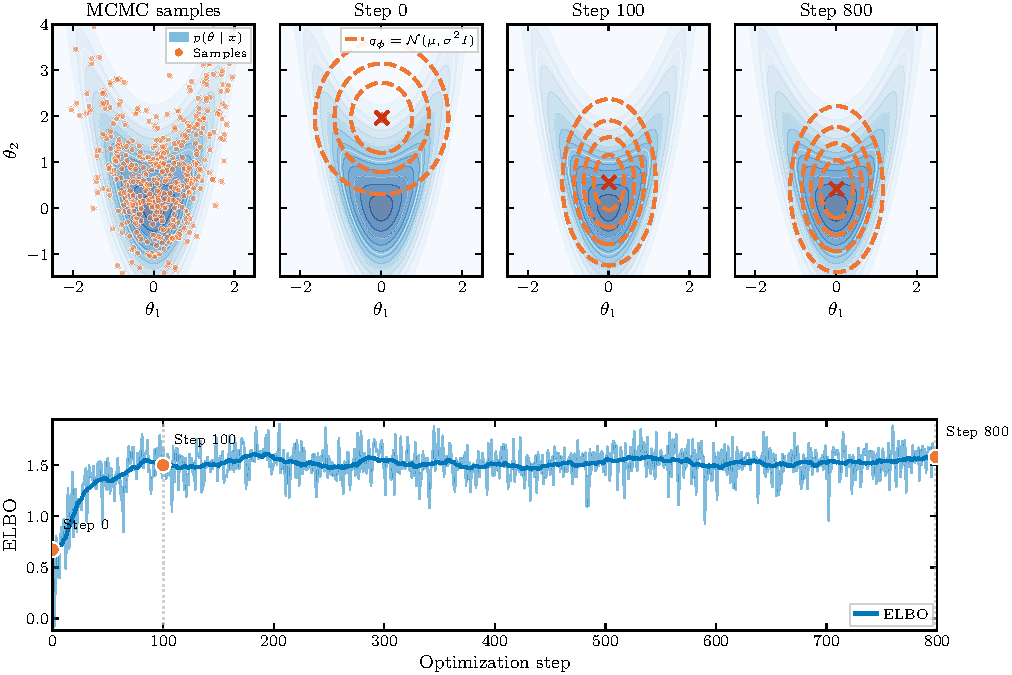
\includegraphics[width=0.98\textwidth]{mcmc_vs_vi_overview.pdf}
\caption{VI on the banana posterior. (Top left) MCMC samples capture the curved shape. (Top right) Evolution of the mean-field Gaussian $q$ during optimization---it finds the right location but cannot represent the curvature. (Bottom) The ELBO increases during optimization.}
\label{fig:vi_optimization_detail}
\end{figure}

\section{Worked example: banana posterior}

Consider a ``banana'' posterior---curved and non-Gaussian:
\beq
p(\theta_1, \theta_2 \mid x) \propto \exp\left( -\frac{1}{2}\theta_1^2 - \frac{1}{2}(\theta_2 - \theta_1^2)^2 \right)
\eeq
This posterior is curved: $\theta_2$ tends to follow $\theta_1^2$.

We'll approximate it with a \emph{mean-field} Gaussian: $q(\theta) = \mathcal{N}(\theta_1; \mu_1, \sigma_1^2) \cdot \mathcal{N}(\theta_2; \mu_2, \sigma_2^2)$---a product of independent Gaussians, one per parameter. Figure~\ref{fig:vi_optimization_detail} shows VI optimization on this posterior.

The optimized $q^*$ correctly locates the high-probability region. But notice what it misses: the mean-field assumption forces independence, so the curved banana becomes an axis-aligned ellipse. And to avoid placing mass in the low-probability ``wings,'' $q$ shrinks, underestimating uncertainty.

\section{Limitations of VI}

\paragraph{The variational family.} The choice of $\mathcal{Q}$ controls the expressiveness--tractability tradeoff. Mean-field Gaussians are fast but cannot capture correlations---as we saw with the banana. A full-covariance Gaussian captures linear correlations but still misses curvature. More expressive families (normalizing flows) can represent complex posteriors but are harder to optimize.

\paragraph{Mode-seeking.} $\KL(q \| p)$ penalizes $q$ for placing mass where $p$ is small. This makes VI \emph{mode-seeking}: when the posterior is multimodal, $q$ concentrates on a single mode and ignores others (Figure~\ref{fig:mode_seeking}).

\begin{figure}[h]
\centering
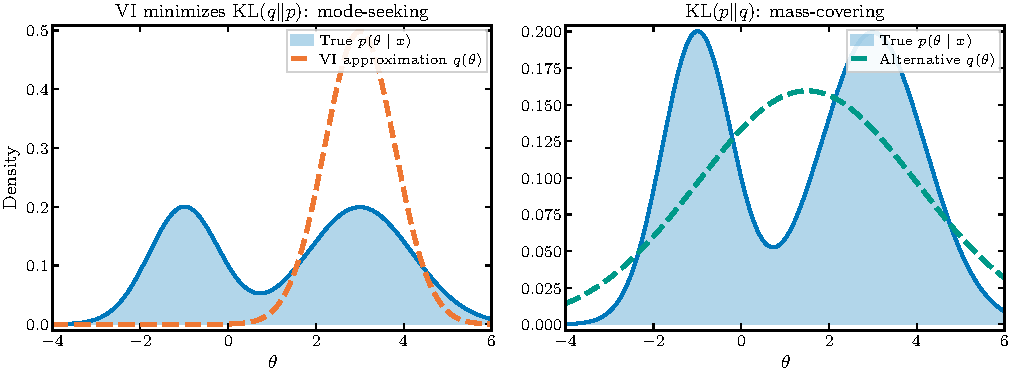
\includegraphics[width=0.8\textwidth]{mode_seeking.pdf}
\caption{Mode-seeking behavior. When the posterior is multimodal, VI concentrates on a single mode rather than covering all modes.}
\label{fig:mode_seeking}
\end{figure}

Because VI is mode-seeking and limited by the variational family, it typically underestimates posterior variance. When accurate uncertainty quantification is critical, MCMC may be the better choice.

\end{document}
